\documentclass[12pt,a4paper, titlepage, openany]{book}
\usepackage{amsmath}
\usepackage{graphicx}
\usepackage{float}
\usepackage{wrapfig}
\usepackage[russian]{babel}
\usepackage[utf8]{inputenc}
\usepackage{geometry}
\geometry{left = 5cm}
\geometry{right = 2cm}



\title{Движение ледокола во льдах}
\date{Долгопрудный - 2022}
\author{Петраков Иван\\\ МФТИ\\\\\\\\\\\\\\\\\\\\}
\hoffset = 0pt
\voffset = 0pt
\textheight = 700pt
\topmargin = 0pt
\headheight = 0pt
\headsep = 0pt
\marginparwidth = 0pt
\oddsidemargin = 0pt
\textwidth = 450pt
\setcounter{tocdepth}{3}

\begin{document}

\maketitle

\tableofcontents

\chapter*{Введение}
\addcontentsline{toc}{chapter}{Введение}

\chapter{Модель среды}
В данной главе описывается модель среды, которая используется в работе.

\section*{Линейно-упругая среда}
Для описания определенных процессов в природе (например, волновых процессов в упругой среде) используется линейная теория упругости, в основе которой лежат два уравнения для описания движения бесконечно-малого объема линейно-упругой среды.\\
Первое уравнение - уравнение движения:
\begin{equation}
\rho \frac{\partial v_i}{\partial t} = \frac{\partial \sigma_{ij}}{\partial x_j}
\end{equation}
где $\rho$ - плотность среды, $v_i$ - компоненты скорости среды в точке, $\sigma_{ij}$ - тензор напряжений Коши.\\
Второе уравнение - реологическое соотношение между деформациями и напряжениями:
\begin{equation}
\begin{aligned}
e_{ij} &= \frac{1}{2}(\frac{\partial u_i}{\partial x_j} + \frac{\partial u_j}{\partial x_i}),\\
\sigma_{ij} &= C_{ijkl} e_{kl}
\end{aligned}
\end{equation}
где $u_i$ - вектор смещения точки тела, $C_{ijkl}$ - тензор упругости, $e_{ij}$ - тензор деформаций.
\\
В нашей модели используется линейно-упругая среда, поэтому тензор упругости зависит только от двух независимых величин $\lambda$ и $\mu$, которые называются параметрами Ламе. Тогда (1.2) можно переписать в виде:
\begin{equation}
\sigma_{ij} = \lambda \delta_{ij} e_{kk} + 2 \mu e_{ij}
\end{equation}
где $\delta_{ij}$ - символ Кронекера. 
\\
Также можно учесть, что тензор деформаций симметричен в силу закона парности касательных напряжений, поэтому если продифференцировать (1.3) по времени, можно получить окончательную систему определяющих уравнений линейно-упругой среды:
\begin{equation}
\begin{cases}
\rho \frac{\partial v_i}{\partial t} = \frac{\partial \sigma_{ij}}{\partial x_j}, \\
\frac{\partial \sigma_{ij}}{\partial t} = \lambda(\frac{\partial}{\partial x_k} v_k) \delta_{ij} + \mu(\frac{\partial v_i}{\partial x_j} + \frac{\partial v_j}{\partial x_i}).
\end{cases}
\end{equation}

\section*{Линейно-акустическая среда}
Помимо описания линейно-упругой среды нам понадобится описание линейно-акустической среды.
\\
Определяющие уравнения линейно-акустической среды получаются из фундаментальных уравнений гидродинамики (уравнение неразрывности и уравнение Эйлера):
\begin{equation}
\begin{aligned}
\frac{\partial \rho}{\partial t} + \nabla \cdot (\rho \mathbf{v}) = \frac{\partial \rho}{\partial t} + \mathbf{v} \cdot \nabla \rho + \rho \nabla \cdot \mathbf{v} &= 0, \\
\frac{\partial \mathbf{v}}{\partial t} + (\mathbf{v} \cdot \nabla) \mathbf{v} + \frac{\nabla p}{\rho} &= 0
\end{aligned}
\end{equation}
где $\rho$ - плотность среды, $\mathbf{v} = (v_x, v_y, v_z)$ - скорость жидкости, $p$ - давление. При этом предполагается, что отклонения плотности, скорости и давления относительно стационарного потока малы:
\begin{equation}
\rho = \rho_0 + \rho', \mathbf{v} = \mathbf{v_0} + \mathbf{v'}, p = p_0 + p'
\end{equation}
\\
Считая, что плотность не зависит от координаты, и тот факт, что стационарый поток должен подчиняться закону сохранения массы, получаем, что поле $\mathbf{v_0}$ должно быть соленоидальным, т.е.
\begin{equation}
\nabla \cdot \mathbf{v_0} = 0
\end{equation}
\\
Подставляя (1.7) и (1.6) в (1.5) получаем:
\begin{equation}
\frac{\partial \rho '}{\partial t} + \mathbf{v_0} \cdot \nabla \rho' + \rho_0 \nabla \cdot \mathbf{v'} = 0.
\end{equation}
\\
В нашей модели считаем процесс распространения малых возмужений адиабатическим, тогда 
\begin{equation}
p' = c^2_p \rho' 
\end{equation}
где
\begin{equation}
c_p = (\frac{\partial p}{\partial \rho})_S
\end{equation}
$S$ - энтропия, $c^2_p = \frac{K}{\rho} = \frac{\lambda}{\rho}$ - скорость акустических волн. Здесь мы воспользовались тем, что в идеальной жидкости нет сдвиговых напряжений и $\mu$ = 0.
\\
Объединяя предыдущие уравнения, получим:
\begin{equation}
\frac{\partial p '}{\partial t} + \mathbf{v_0} \cdot \nabla p' + \lambda \nabla \cdot \mathbf{v'} = 0.
\end{equation}
\\
Осталось получить уравнения для производной по времени малых изменений скорости. Проводим аналогичные действия и получаем:
\begin{equation}
\frac{\partial \mathbf{v'}}{\partial t} + (\mathbf{v_0} \cdot \nabla) \mathbf{v'} + \frac{\nabla p'}{\rho_0} = 0
\end{equation}
\\
Используя связь между нормальными напряжениями и давлением 
\begin{equation}
\sigma_{xx} = \sigma_{yy} = \sigma_{zz} = -p'
\end{equation}
получим итоговую систему для акустоупругой системы в тензорном представлении:
\begin{equation}
\begin{cases}
\rho \frac{\partial v_i}{\partial t} + v^0_k \frac{\partial v_i}{\partial x_k} = \frac{\partial \sigma_{ij}}{\partial x_i}, \\
\frac{\partial \sigma_{ij}}{\partial t} + v^0_k \frac{\partial \sigma_{ij}}{\partial x_k} = \lambda \frac{\partial  v_k}{\partial x_k} \delta_{ij} + \mu (\frac{\partial v_i}{\partial x_j} + \frac{\partial v_j}{\partial x_i})
\end{cases}
\end{equation}
где для акустической системы  $\mu = 0, \mathbf{v_0} \neq 0$, а для упругой - $\mu \neq 0, \mathbf{v_0} =  0$.

\section*{Упруго-пластическая среда}
\subsection*{Основные положения}
Ниже пойдет речь о классической модели упругопластичности, используемой в работе. Рассмотрение ведем в изотермическом приближении.
\\
Характерными особенностями упругопластического поведения являются:
\begin{enumerate}
\item существование диапазона нагрузок, при которых тело ведет себя упруго,
\item существование критерия пластичности (предела текучести), то есть условия, при выполнении которого движение среды происходит по иным законам,
\item отсутствие влияния темпа деформации на возникающие напряжения.
\end{enumerate}
Основными определяющими физическими величинами в теории упруго-пластической среды являются введенные в первой секции главы тензоры напряжений и деформаций. Тензор деформаций складывается из упругой $e_e$ и пластической $e_p$ деформаций. В трехмерном варианте обозначаем тензор деформаций за $\mathbf{E}$.
\\
В качестве критерия пластичности часто задают функцию текучести, которая может зависить как от тензора напряжений $\mathbf{T}$, так и от накопленных пластических деформаций и, возможно, от дополнительных параметров упрочнения $\epsilon$:
\begin{equation}
f(\mathbf{T}, \mathbf{E}_p, \epsilon) = 0
\end{equation}
Рассмотрим идеальный палстический материал, тогда свободная энергия зависит только от упругих деформаций $\psi = \psi(\mathbf{E}_e)$. Определяющее соотношение для тензора напряжений имеет вид (вывод его оставим за кадром):
\begin{equation}
\mathbf{T} = \rho \frac{\partial \psi}{\partial \mathbf{E}_e}
\end{equation}
\\
Неравенство диссипации для пластического течения имеет вид:
\begin{equation}
\mathbf{T}:d\mathbf{E}_p \geq 0
\end{equation}
\\
Положив
\begin{equation}
d\mathbf{E}_p = d \lambda \frac{\partial f}{\partial \mathbf{T}}
\end{equation}
где $d \lambda$ - неопределенный положительный множитель, мы удовлетворим неравенству диссипации. Это выражение называется ассоциированным законом пластического течения.
\\
\subsection*{Условия текучести}
Так мы определили некоторые общие определяющие соотношения для упруго-пластической среды, основанные на деформационной теории пластичности. Но осталось за кадром функция текучести. Различные модели пластичности основаны на различных функциях текучести. Приведем здесь несколько условий текучести.
\subsubsection*{Условие текучести Треска}
Модель трекска предложения для описания пластического поведения металлов. Функция f имеет вид
\begin{equation}
f = \tau - c
\end{equation}
где $\tau$ - максимальное касательное напряжение, $c$ - предел текучести.
\subsubsection*{Условие текучести Кулона-Мора}
Для сыпучих сред появляется необходимость учета внутреннего трения, зависящего от нормальных напряжений, поэтому 
\begin{equation}
f = \tau_n - \sigma_n tg \phi - c,
\end{equation}
где $\tau_n$ и $\sigma_n$ - касательное и нормальное напряжения на одной площадке с нормалью $\mathbf{n}$, $c$ - сцепление, $\phi$ - угол внутреннего трения.
\subsubsection*{Условие текучести Мизеса}
В модели Мизеса вместо максимального касательного напряжения, как в модели Треска, используется напряжение Мизеса $q = \sqrt{3/2 \mathbf{T'}:\mathbf{T'}} = \sqrt{3 J^{\sigma}_2 (\mathbf{T'})}$, где величина $\sqrt{J^{\sigma}_2 (\mathbf{T'})}$ называется интенсивностью касательных напряжений.
\\
Функция f имеет вид
\begin{equation}
f = q - c
\end{equation}
Если учесть тот факт, что интенсивность касательных напряжений пропорциональна энергии формоизменения в упругом теле, то можно сформулировать критерий пластичности Мизеса: пластическое течение начинается тогда, когда энергия формоизменения достигает критической величины.
\subsubsection*{Условие текучести Друкера-Прагера}
Условие текучести Друкера-Прагера является обобщение условия текучести Мизеса. Функция текучести имеет вид
\begin{equation}
f = q - kp - c
\end{equation}
где $q$ - напряжение по Мизесу, $p$ - давление, $k$ - коэффициент внутреннего трения.
\subsection*{Соответствие теории течения и деформационной теории пластичности в простом нагружении}
Покажем, что в условиях простого нагружения теория течения идеального упругопластического материала, основанная на критерии Мизеса, дает выражения, характерные для деформационной теории пластичности. Для этого подставим функцию текучести Мизеса в ассоциированный закон течения. Тогда
\begin{equation}
\frac{\partial f}{\partial T_{ij}} = \frac{\partial q}{\partial T_{ij}} = \frac{1}{2 q} (T_{km} \frac{\partial T_{km}}{\partial T_{ij}} - \frac{1}{3}T_{ss}\frac{\partial T_{ss}}{\partial T_{ij}})
\end{equation}
Вычисляя первую и вторую производную, получим
\begin{equation}
\begin{cases}
T_{km}\frac{\partial T_{km}}{\partial T_{ij}} = T_{ij}, \\
\frac{\partial T_{ss}}{\partial T_{ij}} = \delta_{ij}
\end{cases}
\end{equation}
\\
Окончательно, 
\begin{equation}
\frac{\partial f}{\partial T_{ij}} = \frac{1}{2 q} T'_{ij}
\end{equation}
\\
Таким образом, на поверхности текучести, где $q = c$, справедливо
\begin{equation}
d\mathbf{E'}_p = \frac{d\lambda}{2 c} \mathbf{T'}
\end{equation}
\\
Полученное уравнение называется законом пластического течения Прандтля-Рейса.
\\
Величина $d  \lambda$ пропорциональна работе $d A_p$ девиатора напряжений $\mathbf{T'}$ на девиаторе пластических деформаций $d\mathbf{E'}_p$:
\begin{equation}
\delta A_p = c d\lambda
\end{equation}
\\
Тогда закон пластического течения примет вид:
\begin{equation}
d\mathbf{E'}_p = \frac{\delta A_p}{2 c^2} \mathbf{T'}
\end{equation}
\\
При реализации простого нагружения оси тензора напряжений неизменны, и при этом согласно критерию Мизеса $\mathbf{T'}:\mathbf{T'} = const$, тогда $\mathbf{T'} = const$. Тогда
\begin{equation}
\mathbf{E'}_p = \frac{A_p}{2 c^2}  \mathbf{T'}
\end{equation}
\\
Обозначая $k = A_p/2c^2$. получим, что деформационная теория и теория пластического течения при простом нагружении совпадают. Поэтому в работе имеем право использовать модель Прандтля-Рейса с условием текучести Мизеса.

\chapter{Численный метод. Разрывный метод Галёркина}

\chapter{Взаимодействие ледовых образований с ледоколом}
\section*{Реология льда}

\section*{Особенности численного решения}

\section*{Двумерная задача}
\subsection*{Постановка}
\par
Рассматривается серия тестовых расчетов в двумерной постановке. Тело с определенной геометрией "носа" контактирует с ледяным полем, размером $1.5 \times 10$м. Тело движется с некоторой начальной скоростью без учета сил сопротивления (в вакууме). Рассматриваются острый и скругленный вариант "носа".
\par
Использовались следующие параметры льда: $E$ = 5 ГПа, $G$ = 1.87 ГПа, $\rho$ = 920 кг/м$^3$. Предел прочности на растяжение $\sigma_T$ = 1.2 МПа, порог пластичности $k_0$ = 0.22 МПа. Параметры для налетающего тела: $E$ = 200 ГПа, $G$ = 75 ГПа, $\rho$ = 7500 кг/м$^3$. Соударения происходили с разными скоростями для возможности отслеживания изменения напряжение на конце "носа". 
\begin{figure}[h]
\begin{minipage}[h]{0.5\linewidth}
\center{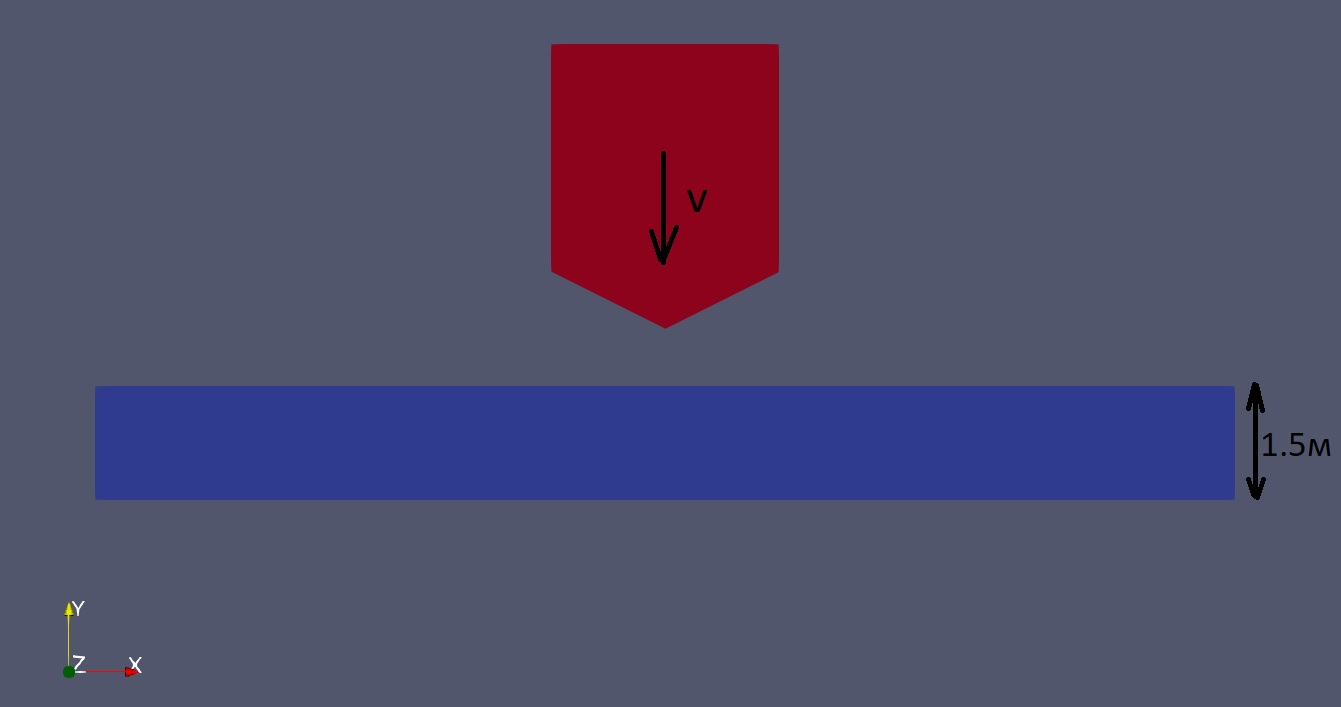
\includegraphics[width=1\linewidth]{task_ship.jpg} \\ (a) Острый нос}
\end{minipage}
\hfill
\begin{minipage}[h]{0.5\linewidth}
\center{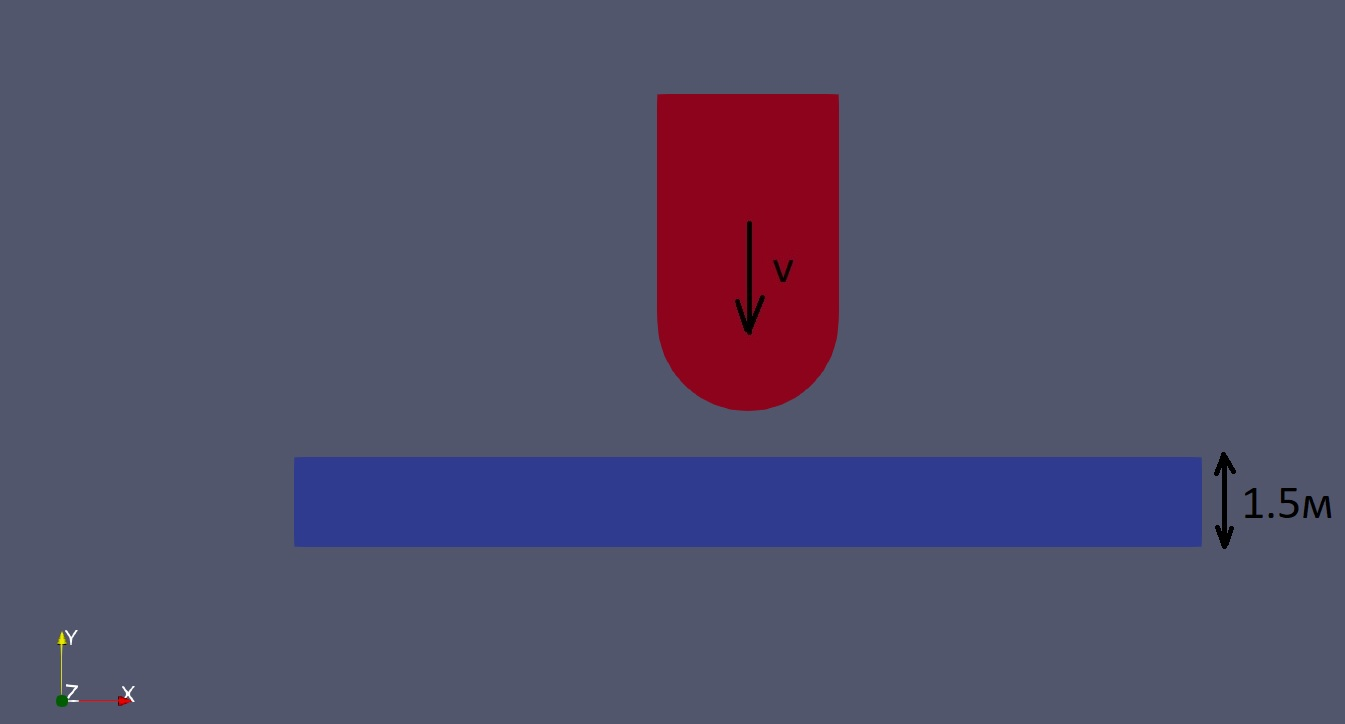
\includegraphics[width=1\linewidth]{task_circle_ship.jpg} \\ (b) Скругленный нос}
\end{minipage}
\caption{Постановка двумерной задачи}
\label{ris:image1}
\end{figure}
\par
На всевозможных граничных ячейках было задано условие свободной границы. Между внутренными ячейками льда и налетающего тела использовалось полное слипание, а на контактной границе "лед-тело" использовалось свободное скольжение. 
\subsection*{Результаты расчетов}

\section*{Трехмерная задача}

\chapter*{Заключение}

\chapter*{Список иллюстраций}

\chapter*{Список таблиц}

\chapter*{Список литературы}

\end{document}